\documentclass[graybox]{svmult}

% -----------------------------------------------------------------------------------

% choose options for [] as required from the list % in the
% Reference Guide

\usepackage{mathptmx}       % selects Times Roman as basic font
\usepackage{helvet}         % selects Helvetica as sans-serif font
\usepackage{courier}        % selects Courier as typewriter font
\usepackage{type1cm}        % activate if the above 3 fonts are
                            % not available on your system
%
\usepackage{makeidx}         % allows index generation
\usepackage{graphicx}        % standard LaTeX graphics tool
                             % when including figure files
\usepackage{multicol}        % used for the two-column index
\usepackage[bottom]{footmisc}% places footnotes at page bottom
\usepackage{seqsplit}
\graphicspath{{Figure/}}

% -----------------------------------------------------------------------------------

\usepackage[table,xcdraw]{xcolor}
\usepackage{xcolor, soulutf8}
\newcommand{\highlight}[1]{\colorbox{yellow!50}{#1}}

\usepackage{amsmath}
% \usepackage{amssymb}         % for additional mathematical symbols
\usepackage{amsfonts}        % for sets like \mathbb{N}, \mathbb{Z}, etc.
\usepackage{pgfplots}
\pgfplotsset{compat=1.17}

\usepackage{tikz}
\usetikzlibrary{shapes.geometric, arrows}

\tikzstyle{startstop} = [ellipse, minimum width=3cm, minimum height=1cm, text centered, draw=black]
\tikzstyle{process} = [rectangle, minimum width=3cm, minimum height=1cm, text centered, draw=black]
\tikzstyle{data} = [trapezium, trapezium left angle=70, trapezium right angle=110, minimum width=1cm, minimum height=1cm, text centered, draw=black]
\tikzstyle{arrow} = [thick,->,>=stealth]

\usepackage{bm}              % for bold symbols
\usepackage{caption}         % for controlling figure/table captions
\usepackage{float}           % to improve figure positioning

\usepackage[none]{hyphenat} % Prevents hyphenation
\sloppy % Allows LaTeX to be less strict about line breaking


% \usepackage{hyperref}
% \usepackage{apacite}
\usepackage[style=apa, backend=biber]{biblatex}
\addbibresource{references.bib}


\usepackage{enumitem} 
\usepackage[small,compact]{titlesec} 
\titlespacing{\section}{0pt}{*4}{*1.5}

\usepackage{setspace}
\edef\restoreparindent{\parindent=\the\parindent\relax}
\usepackage{parskip}
\restoreparindent

% % custom packages
\usepackage{array}
\usepackage{tabularx}
\usepackage{tabularray}
\usepackage{lineno}

\usepackage{scrextend} 
\usepackage{multirow}			% Multirow tables
\usepackage{subfig}

% to typeset URLs, URIs, and DOIs
\usepackage{url}
\usepackage{mathtools}
%  \usepackage[dvips]{graphicx}
%  \usepackage{epsfig}
 \usepackage{epsf}
% \usepackage{subfigure}
\usepackage{indentfirst}

%% The amssymb package provides various useful mathematical symbols
\renewcommand\tabularxcolumn[1]{m{#1}}
\newcommand{\itemEq}[1]{%
        \begingroup%
        \setlength{\abovedisplayskip}{0pt}%
        \setlength{\belowdisplaayskip}{0pt}%
        \parbox[c]{\linewidth}{\begin{flalign}#1&&\end{flalign}}%
        \endgroup}
\newcolumntype{Y}{>{\centering\arraybackslash}X}

% see the list of further useful packages % in the Reference Guide

\makeindex             % used for the subject index
                       % please use the style svind.ist with
                       % your makeindex program

%%%%%%%%%%%%%%%%%%%%%%%%%%%%%%%%%%%%%%%%%%%%%%%%%%%%%%%%%%%%%%%%%%%%%%%%%%%%%%%%%%%%%%%%%

\begin{document}

\title*{Application of Public Key Encryption on Fuzzy Images in a Company's Security Model}
\titlerunning{Application of Public Key Encryption on Fuzzy Images in a Company's Security Model}

\author{}
\authorrunning{}

\institute{}

\maketitle

\abstract*{
    This report presents an approach to addressing the implementation of a
    security model in companies by using picture fuzzy public key encryption, with a more
    detailed focus on utilizing user biometric data as a secret key. Since biometric data is
    blurred or noisy and changes with each collection, traditional public key encryption
    models cannot be used; instead, a picture fuzzy public key encryption model must be
    employed. This study introduces the concept of picture fuzzy public key encryption
    (PFPKE), a public encryption model that accepts a portion of blurred data (a noisy version
    of the original biometric data) as a private key for decrypting the ciphertext. Unlike
    traditional public key encryption models, where the private key is typically stored on
    devices (e.g., on USB drives), the picture fuzzy public key encryption model does not
    require any device to store the private key
}

\abstract{
    This report presents an approach to addressing the implementation of a
    security model in companies by using picture fuzzy public key encryption, with a more
    detailed focus on utilizing user biometric data as a secret key. Since biometric data is
    blurred or noisy and changes with each collection, traditional public key encryption
    models cannot be used; instead, a picture fuzzy public key encryption model must be
    employed. This study introduces the concept of picture fuzzy public key encryption
    (PFPKE), a public encryption model that accepts a portion of blurred data (a noisy version
    of the original biometric data) as a private key for decrypting the ciphertext. Unlike
    traditional public key encryption models, where the private key is typically stored on
    devices (e.g., on USB drives), the picture fuzzy public key encryption model does not
    require any device to store the private key
}

\keywords{Picture fuzzy public key encryption, fuzzy data, biometrics}

\section{Introduction}
In traditional security models within companies that utilize public key infrastructure (PKI), each employee is required to have a unique public-private key pair. This key pair is essential for secure communication within the organization. When an employee receives an encrypted message, it indicates that the message has been encrypted using the employee’s public key. To decrypt and read the message, the employee must use their private key. The security of the entire system hinges on the confidentiality of the private key. If the private key is compromised, the security of the system is at risk. Therefore, it is crucial for employees to keep their private keys secure.

A widely accepted method for securing private keys is to store them on physical devices such as smart cards or USB drives. These devices require the employee to remember a password to activate the private key. This method, as discussed by \citeauthor{Ellison2000} (\citeyear{Ellison2000}), adds an additional layer of security by combining something the employee has (the physical device) with something they know (the password).

An ideal approach to enhance security further is to use biometric data, such as fingerprints or iris patterns, as a private key. Biometric data is unique to each individual, making it a convenient and secure way to serve as a private key for users. \citeauthor{Connaughton2007} (\citeyear{Connaughton2007}) highlight the advantages of using biometric data, noting that it eliminates the need for employees to remember passwords or carry physical devices. However, biometric data can be blurry or noisy and may change slightly each time it is captured. This variability makes it unsuitable for use as a private key in traditional public key encryption schemes.

To address this issue, this paper introduces the concept of fuzzy signatures, as proposed by \citeauthor{Takahashi2015} (\citeyear{Takahashi2015}). Fuzzy signatures use biometric data as a private key without requiring any additional assistance. This approach leverages the inherent variability in biometric data to create a secure and reliable method for encryption and decryption. \citeauthor{Dodis2008} (\citeyear{Dodis2008}) further elaborate on the use of fuzzy signatures, explaining how they can generate strong cryptographic keys from noisy data.

By applying public key cryptography with fuzzy images, as suggested by \citeauthor{Son2016} (\citeyear{Son2016}), internal company security models can effectively utilize biometrics. This method ensures that even if the biometric data is not captured perfectly every time, the system can still function securely. The use of fuzzy signatures and fuzzy images provides a robust solution for integrating biometric data into public key infrastructure, enhancing the overall security of the system.

This approach not only simplifies the process for employees but also strengthens the security framework of the organization by leveraging the unique and immutable characteristics of biometric data.

\section{Related Work}
\subsection{The research of public-key cryptography}
\citeauthor{diffie1976} (\citeyear{diffie1976}) proposed two kinds of contemporary developments in cryptography are examined, widening applications of teleprocessing have given rise to a need for new types of cryptographic systems, which minimize the need for secure key distribution channels and supply the equivalent of a written signature.
\citeauthor{diffie1988} (\citeyear{diffie1988}) described the development of public-key cryptography and its  principles are elucidated, the discussion covers exponential key exchange, the trap-door knapsack public-key cryptosystem.
\citeauthor{barnes2022} (\citeyear{barnes2022}) describes a scheme for  hybrid public key encryption (HPKE). This scheme provides a variant of public key encryption of arbitrary-sized plaintexts for a recipient public key.
\citeauthor{elgamal1985} (\citeyear{elgamal1985}) addressed new signature scheme is proposed, together with an  implementation of the Diffie-Hellman key distribution scheme that achieves a public key cryptosystem.
\citeauthor{cheon2015} (\citeyear{cheon2015}) introduced a method to reduce the degree of the exponentiation circuit at the cost of additional public keys to accelerate the homomorphic evaluation of the PKE decryption.
\citeauthor{azam2021} (\citeyear{azam2021}) prove that their fast and secure public-key image encryption scheme has a computational complexity that is a polylogarithmic function of the size of the plain text.
In other words, the computational complexity of our scheme is independent of the point generation over
\citeauthor{zhang2021} (\citeyear{zhang2021}) described a data mixing method for encrypting a plaintext block using a block encryption algorithm (such as Elliptic Curve, RSA, etc.) having a block size smaller than that of the plaintext block.
\citeauthor{wee2012} (\citeyear{wee2012}) presented efficient public-key encryption schemes resilient against linear related key attacks (RKA) under standard assumptions and in the standard model. They obtain encryption schemes based on hardness of factoring, BDDH and LWE that remain secure even against an adversary that may query the decryption oracle on linear shifts of the actual secret key.
\citeauthor{hou2023} (\citeyear{hou2023}) introduced a new cryptographic primitive called public key encryption with public-verifiable decryption delegation (PKE-PV D 2), that enables the original decryptor to transmit the decryption key for a specific ciphertext to a designated recipient in a way that is both public-verifiable and privacy-preserving.
\citeauthor{imam2022} (\citeyear{imam2022}) proposed scheme uses four random large prime numbers to generate public–private key pairs and applies XOR operation along with the more complex intermediate process in key-generation encryption and decryption phases to achieve higher algorithm complexity, which would require more time to break the proposed cipher and would make it extremely difficult for third-parties to attack, hence boosting security.

\subsection{The research of biometrics as an security methods and its application in company}
Biometrics such as fingerprints, handprints have been use since ancient times according to \citeauthor{gupta2008biometrics} (\citeyear{gupta2008biometrics}) and the author pointed out the use of biometrics for identity authentication and identification for enhancing security in organizations.
In the research of \citeauthor{bidgoli2012introduction}(\citeyear{bidgoli2012introduction}) has introduced a six-step guide for company using biometrics as a security measure.
\citeauthor{naganuma2020new} (\citeyear{naganuma2020new}) has published a study about using biometrics fuzzy signature as a secret key management based on Blockchain technology as an innovative system for decentralized payments in fields such as financial area.
\citeauthor{chang2004biometrics} (\citeyear{chang2004biometrics}) proposed a biometrics-based cryptographic key generation framework to advoid the vulnerability to be dictionary attacked by using PINs and passwords.
\citeauthor{sengel2020efficient} (\citeyear{sengel2020efficient}) pointed out that the security performance of substitution box using fingerprint patterns is an successful algorithm promising to be used in mobile devices.
\citeauthor{dhir2019uidba} (\citeyear{dhir2019uidba}) proposed an architecture, which focus on fingerprint driven digital signing in order to replace existing business processes within Governments with transparent and accountable technology driven transactions.
\citeauthor{jin2016biometric} (\citeyear{jin2016biometric}) propose an ECC-free key binding scheme along with cancellable transforms for minutiae-based fingerprint biometrics, the minutiae information is favorably protected by a strong non-invertible cancellable transform, which is crucial to prevent a number of security and privacy attacks.
\citeauthor{song2007personalized} (\citeyear{song2007personalized}) addressed Fingerhashing approach which transforms fingerprint into a binary discretized representation called Fingerhash and aimed to clarify some of the practical and security problems when using fingerhash to secure biometric key for protecting digital contents, they study two existing directions of biometric‐based key generation approach based on the usability, security and accuracy aspects.
\citeauthor{nivedetha2020ffbks} (\citeyear{nivedetha2020ffbks}) published  experimental results show that the proposed Fuzzy Fingerprint Biometric Key Based Security Schema achieves better performance compared with the existing system in terms of simulation time, energy consumption, delay and attack detection rate.
\citeauthor{kaur2023biometric} (\citeyear{kaur2023biometric}) combines characteristics of both the fields: biometric and cryptosystem, where biometric provides authentication and cryptosystem imparts security called Biometric Cryptosystem (BCS), BCS is prone to various attacks and this study covers 30 such attacks, its countermeasures to thwart these attacks.
\\[6pt]

\subsection{The research of picture fuzzy public key encryption in security}
\citeauthor{bellare2006relations} (\citeyear{bellare2006relations}) compare the relative strengths of popular notions of security for public key encryption schemes and consider the goals of privacy and non-malleability, each under chosen plaintext attack and two kinds of chosen ciphertext attack.
\citeauthor{cramer1998practical} (\citeyear{cramer1998practical}) proposed a new public key cryptosystem is proposed and analyzed.
The scheme is practical, and is provably secure against adaptive chosen ciphertext attack under standard intractability assumptions.
\citeauthor{naor1990public} (\citeyear{naor1990public}) construct a public-key cryptosystem secure against chosen ciphertezt attacks, given a public-key cryptosystern secure against passive eavesdropping and a noninteractive zero-knowledge proof system in the shared string model.
\citeauthor{fujisaki1999enhance} (\citeyear{fujisaki1999enhance}) presented a simple and efficient conversion from a semantically secure public-key encryption scheme against passive adversaries to a non-malleable (or semantically secure) public-key encryption scheme against adaptive chosenciphertext attacks (active adversaries) in the random oracle model.
\citeauthor{okamoto1998new} (\citeyear{okamoto1998new}) published a paper address a novel public-key cryptosystem, which is practical, provably secure and has some other interesting properties.
\citeauthor{blum1985efficient} (\citeyear{blum1985efficient}) introduced first probabilistic public-key encryption scheme which combines perfect secrecy with respect to polynomial time eavesdroppers and eficiecy, in order that enhance the security of the system.
\citeauthor{canetti2003forward} (\citeyear{canetti2003forward}) presented the first constructions of a (non-interactive) forward-secure public-key encryption scheme, their construction achieves security against chosen plaintext attacks under the decisional bilinear Diffie-Hellman assumption in the standard model.
It is practical, and all complexity parameters grow at most logarithmically with the total number of time periods.
The scheme can also be extended to achieve security against chosen ciphertext attacks.
\citeauthor{dolev1983security} (\citeyear{dolev1983security}) used public key encryption to provide secure network communication has received considerable attention.
\citeauthor{agrawal2023public} (\citeyear{agrawal2023public}) introduce the notion of public key encryption with secure key leasing (PKE-SKL).
\citeauthor{chen2016dual} (\citeyear{chen2016dual}) investigate the security of a well-known cryptographic primitive, namely, public key encryption with keyword search (PEKS) which is very useful in many applications of cloud storage and provide an efficient instantiation of the general framework from a Decision Diffie–Hellman-based LH-SPHF and show that it can achieve the strong security against inside the KGA.

\section{Symbols and definitions}
\begin{enumerate}[label=(\roman*), itemsep=1em]
    \item Let \( \mathbb{N} \), \( \mathbb{Z} \), and \( \mathbb{R} \) denote the sets of natural numbers, integers, and real numbers, respectively. If \( n \in \mathbb{N} \), let \( [n] := \{1,\, \ldots,\, n\} \). If \( a \in \mathbb{R} \), then \( \boldsymbol{\lfloor a \rceil} \) denotes the nearest integer to \( a \). Additionally, if \( a = \boldsymbol{(a_1,\, a_2,\, \ldots)} \), let \( \boldsymbol{\lfloor a \rceil := (\lfloor a_1 \rceil,\, \lfloor a_2 \rceil,\, \ldots)} \).
    \item The notation \( x \leftarrow y \) denotes that \( y \) is assigned to \( x \). If \( S \) is a finite set, \( |S| \) represents its size, and \( x \leftarrow_{\mathbf{R}}   S \) means that \( x \) is chosen randomly from \( S \). If \( \varPhi \) is a distribution over some set, \( x \leftarrow_{\mathbf{R}} \varPhi \) denotes that \( x \) is chosen according to distribution \( \varPhi \). Let \( f: D \rightarrow R \) be a function and \( y \in R \) a value; \( \boldsymbol{ f^{-1}(y) } \) represents the set of pre-images of \( y \) under \( f \), i.e., \( \boldsymbol{ f^{-1}(y) := \{x \in D \mid f(x) = y\} } \). If \( x \) and \( y \) are bitstrings, then \( |x| \) denotes the bit length of \( x \), and \( (x || y) \) represents the concatenation of \( x \) and \( y \).
    \item A function \( f(.): \mathbb{N} \rightarrow [0, 1] \) is called negligible if for every positive polynomial \( p(.) \) and every sufficiently large \( \mathbf{\lambda} \) then \(  \mathbf{f(\lambda) < \dfrac{1}{p(\lambda)}} \).
    \item How to set the open key: \\
          1 open key setting \( \mathbf{F} \) includes \( ((d, \, X), \, t, \, \mathcal{X}  ,\, \varPhi,\, \mathbf{\epsilon} ) \) with \( (d, \, X) \) being the spatial data with \( X \) being the space containing the values of the fuzzy set of the picture \( A \) and \( d :\mathbf{X^2} \to \mathbb{R} \) being the corresponding distance function. \( t \in \mathbb{R} \) is the threshold value determined by the security parameter \( \lambda \), \( \mathcal{X} \) is the distribution of the fuzzy data on \( X \), \( \varPhi \) is the error distribution and \( \mathbf{ \epsilon \in [0,1] } \) is an error parameter representing the false rejection rate. The False Acceptance Rate (FAR) and False Rejection Rate (FRR) are determined based on the threshold value \( t \).\\[6pt]
          \textbf{Requirement}: \( \text{FAR} := \Pr[x,\, x' \leftarrow_{\mathbf{R}} {\mathcal{X}} : d(x,\, x') < t] \) is negligible in the security parameter  \( \lambda \). Also for all fuzzy data parts of \( x \in \mathbf{X} \), \( \text{FRR} := \Pr[e \leftarrow_{\mathbf{R}} \varPhi : \mathrm{d}(x, \, x + e) \geq t] \leq \epsilon \)
    \item The definition of picture fuzzy set (PFS) is an extension of fuzzy set and intuitionistic fuzzy set. Picture fuzzy set is based on a complete model in situations where we have human opinions: yes, no, neutral. \\[6pt]
          Given a background set \( X = \{x_1, x_2, \dots, x_n \} \), a picture fuzzy set \( A \) on \( X \) is defined by
          \begin{equation}
              A = \left\{ \langle x,\, \mu_A(x),\, \eta_A(x),\, \nu_A(x) \rangle \mid x \in X \right\}
          \end{equation}

          Where:
          \begin{align}
              \mu_A  & : X \to [0, 1] \quad \text{is a positive function} \\[6pt]
              \eta_A & : X \to [0, 1] \quad \text{is a neutral function}  \\[6pt]
              \nu_A  & : X \to [0, 1] \quad \text{is a negative function}
          \end{align}

          Satisfy the condition:
          \begin{equation}
              \mu_A(x) + \eta_A(x) + \nu_A(x) < 1 \quad \forall x \in X
          \end{equation}

          Apply the \( L- R \) fuzzy number formula to calculate \( \mu(x) = \langle b, c \rangle \), where \( b \) is the average value in set \( X \), and \( c \) is the maximum value in set \( X \):
          \begin{equation}
              \mu(x) = \begin{cases}
                  0                & \text{if } x \leq c     \\
                  \dfrac{x-b}{c-b} & \text{if } b < x \leq c
              \end{cases}
          \end{equation}

          Apply the triangular fuzzy number formula to calculate \( \eta(x) = \langle a, b, c \rangle \), where \( b \) is the average value in the set \( X \):
          \begin{align}
              a       & = \dfrac{b + \min(X)}{2}                                          \\[6pt]
              c       & = \dfrac{b + \max(X)}{2}                                          \\[6pt]
              \eta(x) & = \begin{cases}
                              0                & \text{if } x \geq c \text{ or } x < a \\
                              \dfrac{c-x}{c-b} & \text{if } b \leq x < c               \\[6pt]
                              \dfrac{x-a}{b-a} & \text{if } a \leq x < b
                          \end{cases}
          \end{align}


          Apply the \( L - R \) fuzzy number formula to calculate \( \nu(x) = \langle a, b \rangle \), where \( b \) is the average value in set \( X \), and \( a \) is the minimum value in set \( X \):
          \begin{equation}
              \nu(x) = \begin{cases}
                  0                & \text{if } x \geq a     \\
                  \dfrac{b-x}{b-a} & \text{if } a \leq x < b
              \end{cases}
          \end{equation}

\end{enumerate}


\begin{figure}[H]
    \centering
    \begin{tikzpicture}
        \begin{axis}[
                width=12cm, % Scale the plot to desired width
                height=5.5cm,
                axis lines=middle,
                xmin=0, xmax=10,
                ymin=0, ymax=1.2,
                xlabel={},      % Empty string to hide x-axis label
                ylabel={},      % Empty string to hide y-axis label
                xtick={0, 2, 4, 6, 8},
                ytick={0, 0.2, 0.4, 0.6, 0.8, 1},
                yticklabel style={/pgf/number format/.cd, fixed, precision=1},
                domain=0:10,
                samples=100,
                smooth,
                clip=false
            ]

            % Draw the sigmoid curve
            \addplot[thick, domain=0.4:8] {1/(1 + exp(-1.21 * (x - 4.2)))};

            % Dashed lines for the points a, b, c
            \draw[dashed] (axis cs:4.2,0) -- (axis cs:4.2,0.5) -- (axis cs:0,0.5);
            \draw[dashed] (axis cs:8,0) -- (axis cs:8,1) -- (axis cs:0,1);

            % Labels for points a, b, c with adjusted positions
            \node[below=15pt] at (axis cs:4.2,0) {\( b \)};
            \node[below=15pt] at (axis cs:8,0) {\( c \)};
            \node[below=15pt] at (axis cs:0.5,0) {\( a \)};
            \node[left=2pt] at (axis cs:0,1.2) {1.2};
            \node[below=2pt] at (axis cs:10,0) {10};

        \end{axis}
    \end{tikzpicture}
    \caption{Membership functions applied to high level of security of fuzzy sets of pictures}
    \label{fig:membership_function_security_analysis}
\end{figure}

\section{Famework and security model of public key cryptography of watermark}
\subsection*{A. Framework of Public Key Cryptography for Watermark}

The public key cryptography scheme consists of the following six algorithms: Key Extraction, Setup Algorithm, Key Generation Algorithm, Encrypt Algorithm, and Decrypt Algorithm:

\begin{itemize}
    \item \textbf{Extract the fuzzy picture (Bio)}
          \begin{equation}
              \{ \langle x,\, \mu_A(x),\, \eta_A(x),\, \nu_A(x) \rangle \mid x \in X \}
          \end{equation}
          When entering the user's biometric information, the algorithm will output the fuzzy picture data.

    \item \textbf{Set} \( (1^\lambda) \to par  \): when entering the security parameter \( \lambda \), this algorithm will output the public parameter \(  par \), including the fuzzy key setting
          \begin{equation}
              F = ((d, \, X), \, t, \, \mathcal{X}, \, \varPhi, \, \epsilon)
          \end{equation}

    \item \textbf{KeyGen} \( (par ,\, x) \to \text{pk}_f \): when entering the public parameter \(  par \) and the fuzzy picture data of \( x \in X \), this algorithm outputs the public key \( \text{pk}_f \).

    \item \textbf{Encryption} \( (par ,\, \text{pk}_f,\, M) \to \text{CT} \): When entering the public parameter \(  par \), the public key \( \text{pk}_f \) and the message \( M \) (in the message space), this algorithm outputs the ciphertext \( \text{CT} \).

    \item \textbf{Extract the fuzzy picture (Bio)}
          \begin{equation}
              \{ \langle x', \mu_A(x'), \eta_A(x'), \nu_A(x') \rangle \mid x' \in X \}
          \end{equation}
          When entering the user's biometric information, the algorithm will output the fuzzy picture data.

    \item \textbf{Decrypt} \( (par , \text{pk}_f, x', \text{CT}) \to M/\perp \): When entering the public parameter \(  par \), the public key \( \text{pk}_f \), the fuzzy picture data of \( x' \in X \), and the ciphertext \text{CT}, this algorithm outputs the message \( M \) or the error symbol \( \perp \).

\end{itemize}

We say that the public key encryption scheme of a fuzzy picture with the fuzzy key setting \( F \) is correct, meaning that for every security parameter \( \lambda \in \mathbb{N} \) with all fuzzy picture data of \( x, x' \in X \) such that \( \mathrm{d}(x, x') < t \), for all messages \( M \) in the message space, if:
\begin{align}
    par         & \leftarrow \text{Set}(1^\lambda)                    \\[6pt]
    \text{pk}_f & \leftarrow \text{KeyGen}(par ,\, x)                 \\[6pt]
    \text{CT}   & \leftarrow \text{Encrypt}(par ,\, \text{pk}_f,\, M)
\end{align}

we get:
\begin{equation}
    \text{Decrypt}(par ,\, \text{pk}_f,\, x',\, \text{CT}) = M
\end{equation}

\subsection*{B. Security Model}

Similar to the security definition of a public key cryptography scheme, a fuzzy public key cryptography scheme is required to be indistinguishable under universal faults of the fuzzy key setting \( F \).
A fuzzy public key cryptography scheme in fuzzy key setting \( F \) is said to be indistinguishable under chosen ciphertext attacks (IND-CCA security) if for any adversary \( \mathcal{A} \) we have an advantage function given by:
{
\small
\begin{equation}
    Adv\begin{array}{c}
        ind-cca                  \\
        \text{FPKE}, \mathcal{A} \\
    \end{array} (\lambda)
    =
    Pr\left[b'= b \left| \begin{array}{c}
            par  \leftarrow Init(1^\lambda)                                                         \\
            x^* \leftarrow_{R} \mathcal{X}, \, b \leftarrow \{0, 1 \}                               \\
            pk^*_f \leftarrow KeyGen(par , \, x^*)                                                  \\

            (M_{0}, \, M_{1}, \, \text{state}) \leftarrow \mathcal{A}^{O_{Dec(.)}}(par , \, pk^*_f) \\
            CT^* \leftarrow Encrypt(par , \, pk^*_f, \, M)                                          \\
            b' \leftarrow \mathcal{A}^{O_{Dec(.)}}(par  , \, pk^*_f, \, M_0, \, M_1, \, \text{state}, \, CT^*)
        \end{array} \right. \right] - \frac{1}{2}
\end{equation}
}
This is negligible in the security parameter \( \lambda \), with \( |M_0| = |M_1| \) and \( O_{\text{DEC}(.)} \) being the decryption guess, taking the public parameter \(  par \), the public key \( \text{pk}_f^* \), a fragment of the watermark data \( x^* \), and a fragment of the ciphertext \( \text{CT} \) as input, and outputting the message \( M \leftarrow \text{Decrypt}(par ,\, \text{pk}_f^*,\, x^*,\, \text{CT}) \).


\section{Construct algorithm for fuzzy public key encryption}
\subsection*{- Encryption Algorithm}
\begin{figure}[H]
    \centering
    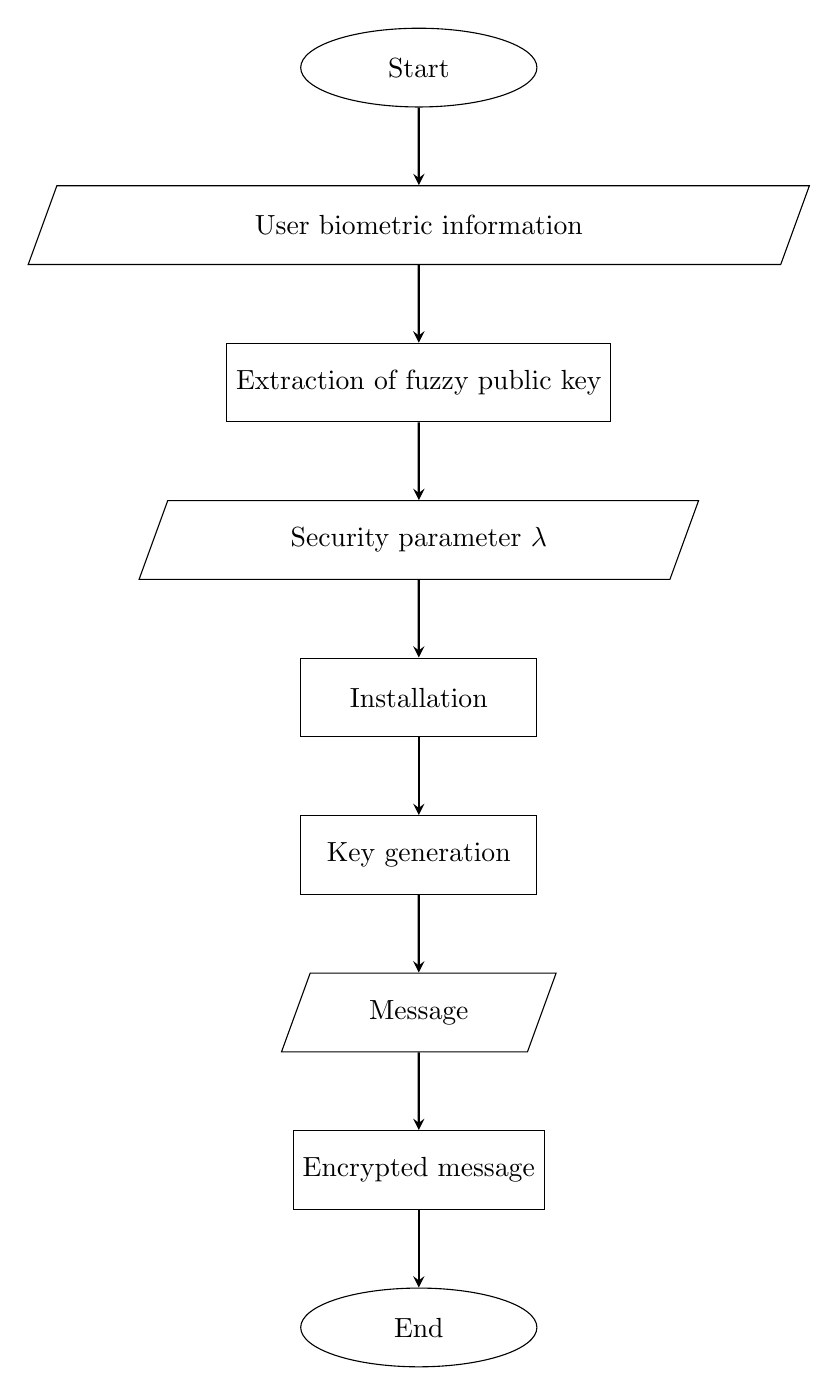
\begin{tikzpicture}[node distance=2cm]
        % Nodes
        \node (start) [startstop] {Start};
        \node (bio) [data, below of=start] {User biometric information};
        \node (fuzzykey) [process, below of=bio] {Extraction of fuzzy public key};
        \node (security) [data, below of=fuzzykey] {Security parameter \( \lambda \)};
        \node (installation) [process, below of=security] {Installation};
        \node (keygen) [process, below of=installation] {Key generation};
        \node (message) [data, below of=keygen] {Message};
        \node (encrypted) [process, below of=message] {Encrypted message};
        \node (end) [startstop, below of=encrypted] {End};

        % Arrows
        \draw [arrow] (start) -- (bio);
        \draw [arrow] (bio) -- (fuzzykey);
        \draw [arrow] (fuzzykey) -- (security);
        \draw [arrow] (security) -- (installation);
        \draw [arrow] (installation) -- (keygen);
        \draw [arrow] (keygen) -- (message);
        \draw [arrow] (message) -- (encrypted);
        \draw [arrow] (encrypted) -- (end);

    \end{tikzpicture}
    \caption{Biometric encryption using picture fuzzy algorithm}
    \label{fig:biometric_encryption_fuzzy}
\end{figure}

Example of the Encryption Algorithm:
\begin{enumerate}[itemsep=1em]
    \item First, the algorithm will perform the extraction of the biometric information of the user that has been encoded into a vector \( x = (5, 7, \dots, 1) \).
    \item Then, it will extract the information of the fuzzy public key \( A = \langle 0.75, 0.1, 0.15 \rangle \).
    \item After that, choose \( \lambda \) as a random number in the range \( \{0, \, 2^{64} - 1\} \) as the input security parameter.
    \item Execute the installation algorithm to obtain the output public parameter:\\
          par =
          \seqsplit{\textquotedblleft MFwwDQYJKoZIhvcNAQEBBQADSwAwSAJBAJQVu6lHAEtia3xc8fCEKd9dpt0jGt7FSiMz\textquotedblright}


    \item With \( par \) and fuzzy public key data obtained above through the key generation algorithm, the output public key \\ \( pk_f = (pk, \, c) \) =
          \seqsplit{(MFwwDQYJKoZIhvcNAQEBBQADSwAwSAJBAKD/RZvqG4ocFdsCpVpUbgrlYlEumD9qebAIVm3gv1Y6XN7w6jf2B4V9soP9jbXcmwEDy/N6xognyuqKAEB81JUCAwEAAQ==, \, MFwwDQYJKoZIhvcNAQEBBQADSwAwSAJBAKNQ0UmtSE2dD6Mbx0Vd8GWcTYvqPJNTqyg7xtJAYWWGPmjScKH1VUZw0lIRve3mtlLoxa7mRntUm6iw94ZSCXcCAwEAAQ).}

    \item Input the message to be encrypted \\ \( M = \text{\textquotedblleft PUBLIC ENCRYPTION OF FUZZY PUBLIC KEY\textquotedblright} \) into the algorithm. From the message to be encrypted and the key obtained above through the encryption algorithm, we obtain the ciphertext:\\ \( CT \)
          =  \seqsplit{\textquotedblleft exhxWbrXSm7huDc/4LkAHnmk3i91K1FDBqUwpk01gLR0pY8Ow/SQe3xPLpdkSpoTLwm/T3KqI0qGs8HehzXHHw==\textquotedblright}.
\end{enumerate}

\begin{figure}[H]
    \centering
    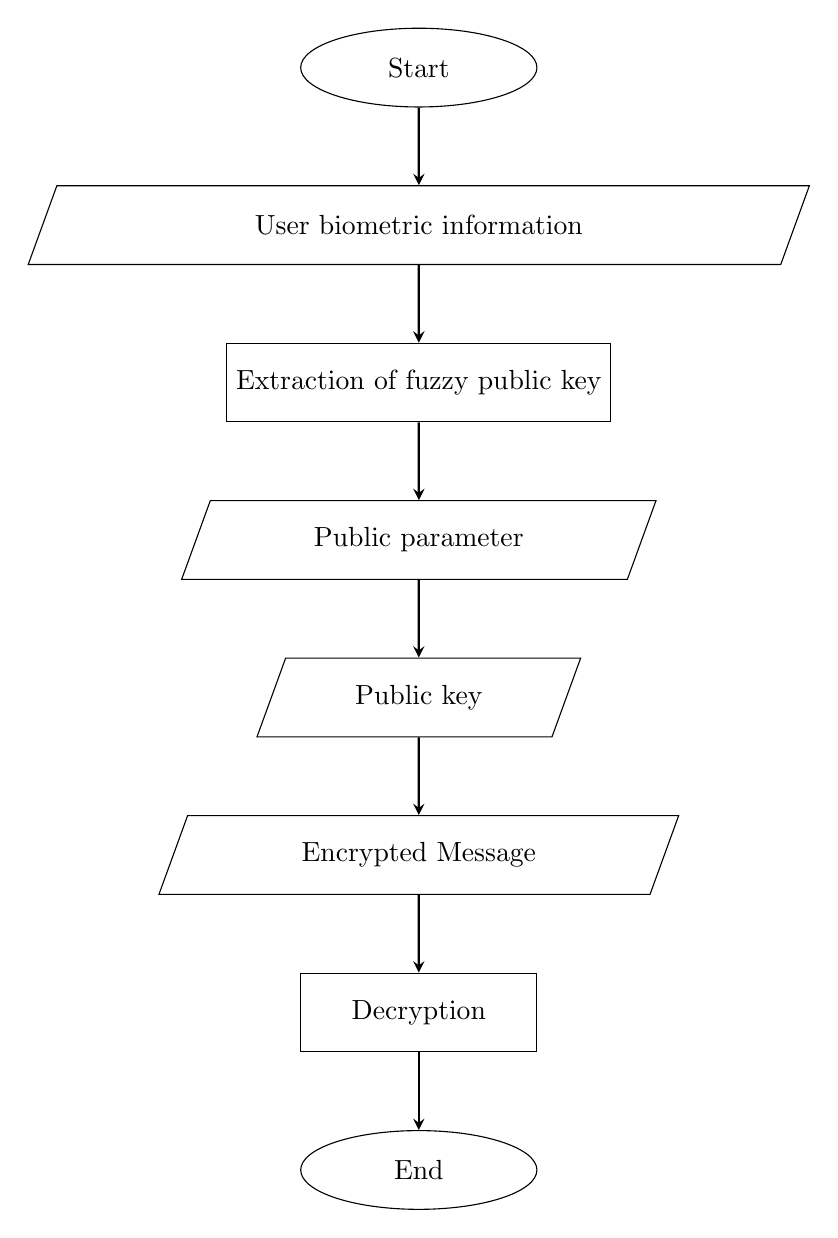
\begin{tikzpicture}[node distance=2cm]
        % Nodes
        \node (start) [startstop] {Start};
        \node (biometric) [data, below of=start] {User biometric information};
        \node (fuzzykey) [process, below of=biometric] {Extraction of fuzzy public key};
        \node (parameter) [data, below of=fuzzykey] {Public parameter};
        \node (publickey) [data, below of=parameter] {Public key};
        \node (message) [data, below of=publickey] {Encrypted Message};
        \node (decryption) [process, below of=message] {Decryption};
        \node (end) [startstop, below of=decryption] {End};

        % Arrows
        \draw [arrow] (start) -- (biometric);
        \draw [arrow] (biometric) -- (fuzzykey);
        \draw [arrow] (fuzzykey) -- (parameter);
        \draw [arrow] (parameter) -- (publickey);
        \draw [arrow] (publickey) -- (message);
        \draw [arrow] (message) -- (decryption);
        \draw [arrow] (decryption) -- (end);

    \end{tikzpicture}
    \caption{Biometric decryption using picture fuzzy algorithm}
    \label{fig:biometric_decryption_fuzzy}
\end{figure}

Example of the Decryption Algorithm:
\begin{enumerate}[itemsep=1em]
    \item First, the algorithm will perform the extraction of the biometric information of the user that has been encoded into a vector \( x' = (5,\, 6, \, \dots, \, 1) \).
    \item Then, it will extract the information of the fuzzy public key. The output will be the data of the fuzzy public key \( A = \langle 0.74,\, 0.1,\, 0.15 \rangle \).
    \item With the input parameters, including the fuzzy public key, the public parameter:
          \\[6pt] \( par \) = \seqsplit{\textquotedblleft MFwwDQYJKoZIhvcNAQEBBQADSwAwSAJBAJQVu6lHAEtia3xc8fCEKd9dpt0jGt7FSiMz\textquotedblright},
          public key:
          \\[6pt] \( pk_f \) = \seqsplit{(MFwwDQYJKoZIhvcNAQEBBQADSwAwSAJBAKD/RZvqG4ocFdsCpVpUbgrlYlEu mD9qebAIVm3gv1Y6XN7w6jf2B4V9soP9jbXcmwEDy/N6xognyuqKAEB81JUCAwEAAQ==, MFwwDQYJKoZIhvcNAQEBBQADSwAwSAJBAKNQ0UmtSE2dD6Mbx0Vd8GWcTYvqPJ NTqyg7xtJAYWWGPmjScKH1VUZw0lIRve3mtlLoxa7mRntUm6iw94ZSCXcCAwEAAQ)},
          \\[6pt] and the code\\ \( CT \) = \seqsplit{\textquotedblleft exhxWbrXSm7huDc/4LkAHnmk3i91K1FDBqUwpk01gLR0pY8Ow/SQe3xPLpdkSpoTL wm/T3KqI0qGs8HehzXHHw==\textquotedblright.}
    \item After the decryption algorithm, we obtain:
          \( M \) = \textquotedblleft PUBLIC KEY ENCRYPTION OF THE FUZZY PUBLIC KEY\textquotedblright.
\end{enumerate}

\subsection*{- Detailed Implementation of the Algorithm}
Install the fuzzy key \( F = ((d, X), t, \mathcal{X}, \varPhi, \epsilon) \). The Public Fuzzy Public Key Encryption (PFPKE) includes extracting the fuzzy representation, installation, Keygen, key code, and decryption, ensuring IND-CCA security, with \( K \) being the space of private keys that determine the key characteristics and homomorphism.

Assume that \( S = (\text{S.Setup},\, \text{S.Sketch}, \text{S.DiffRec}) \) is the probabilistic algorithm for installing the fuzzy key \( F \), and \( \text{Sig} = (\text{Sig.KeyGen},\, \text{Sig.Sign},\, \text{Sig.Verify}) \) is the one-time signature algorithm.

The public-key cryptographic scheme of the fuzzy representation (PFPKE) is linked to the installation of the fuzzy key \( F \), including the following steps:

\begin{enumerate}
    \item \textbf{Extract the fuzzy representation}: This step takes the biometric information of the user as input. The output is the fuzzy representation data:
          \begin{equation}
              \text{Gen(Bio)} = \left\{ \langle x,\, \mu_A(x),\, \eta_A(x),\, \nu_A(x) \rangle \mid x \in X \right\}
          \end{equation}

    \item \textbf{Installation}: The security parameter \( \lambda \) is taken as input. It defines the \break installation of the fuzzy key \( F = ((d,\, X),\, t,\, \mathcal{X},\, \varPhi,\, \epsilon) \). The public parameter \(  par \) is obtained:
          \begin{align}
              par_{pke} & \leftarrow_R S.\text{Setup}(1^\lambda) \\[6pt]
              par_S     & \leftarrow_R S.\text{Setup}(\kappa, +)
          \end{align}
          The final public parameter is:
          \begin{equation}
              par  = (par_{pke},\, par_S,\, F).
          \end{equation}

    \item \textbf{KeyGen}: Takes the public parameter \(  par \) and a part of the fuzzy representation data of \( x \) as input. It parses \( par  = (par_{pke}, par_S) \), then runs:
          \begin{align}
              sk & \leftarrow_R \kappa                              \\[6pt]
              pk & \leftarrow \text{KeyGen}(par_{pke}, \, sk)       \\[6pt]
              c  & \leftarrow_R S.\text{Sketch}(par_S, \, sk, \, x)
          \end{align}
          The output is the public key:
          \begin{equation}
              pk_f = (pk,\, c)
          \end{equation}

    \item \textbf{Encryption}: Takes the public parameters \(  par \), the public key \( pk_f \), and the message \( M \) as input. It parses \( par  = ( par_{pke}, \, par_S) \) and \( pk_f = (pk, \, c) \). The signature key generation algorithm is run:
          \begin{equation}
              ssk \leftarrow \text{Sig.KeyGen}(),
          \end{equation}
          generating the signing key $ssk$ and verification key $svk$. The ciphertext $CT$ is obtained by running:
          \begin{equation}
              CT \leftarrow_R \text{Encoding}(par_{pke}, \, pk, \, svk, \, M).
          \end{equation}
          The signature $\sigma$ is created with the signing key $ssk$ on $CT$, and the final output is the encoded message:
          \begin{equation}
              CT = (svk, \, CT, \, \sigma).
          \end{equation}

    \item \textbf{Extract fuzzy representation}: This step takes the user's biometric information as input. The output is the fuzzy representation data:
          \begin{equation}
              \text{Gen}(\text{Bio}) = \left\{ \langle x', \, \mu_A(x'), \, \eta_A(x'), \, \nu_A(x') \rangle \mid x' \in X \right\}.
          \end{equation}

    \item \textbf{Decryption}: Takes the public parameters \(  par \), the public key \( pk_f \), the fuzzy representation data of \( x' \in X \), and the encoded message \( CT \) as input. It parses \( par  = (par_{pke}, par_S) \), \( pk_f = (pk, \, c) \), and \( CT = (svk, \, CT, \, \sigma) \). If \( \sigma \) is the signature on \( CT \) with respect to the public key \( svk \), it will run:
          \begin{align}
              sk' & \leftarrow_R \kappa                              \\[6pt]
              pk' & \leftarrow \text{KeyGen'}(par_{pke}, sk')        \\[6pt]
              c'  & \leftarrow S.\text{Sketch}(par_S, \, sk', \, x')
          \end{align}

          The difference key \( \Delta sk \) is obtained by:
          \begin{equation}
              \Delta sk \leftarrow S.\text{DiffRec}(par_S, \, c, \, c0).
          \end{equation}
          Finally, decryption proceeds as:
          \begin{equation}
              M \leftarrow \text{Decoding}(par_{pke}, \, \Delta sk, \, CT, \, pk', \, sk'),
          \end{equation}
          and the output is the message \( M \).
\end{enumerate}

\section{Some additional properties}
For the public key encryption scheme used to construct the public key encoding of the fuzzy representation, it is necessary to define some additional properties:

\subsection{Key Determination Scheme}

The decision key is the KeyGen algorithm that first randomly selects a key \( sk_{pke} \) (from the secret key space) and calculates the corresponding public key \( pk_{pke} \) (determined by the secret key \( {sk}_{pke} \)) during the key generation process. Formally, a public-key cryptographic scheme is a Key Determination Scheme if the public parameter \( {par}_{pke} \) is generated by a specified set algorithm, specifying the private key space \( \kappa_{pke} \), and there exists a specified algorithm KeyGen' such that the algorithm to generate the key KeyGen can be defined as \( \text{KeyGen}(par_{pke}) \):
\begin{align}
    sk_{pke}       & \leftarrow_R \kappa_{pke}                         \\[6pt]
    pk_{pke}       & \leftarrow \text{KeyGen}'(par_{pke}, \, sk_{pke}) \\[6pt]
    \text{Return } & (sk_{pke}, \, pk_{pke}).
\end{align}

\subsection{Homomorphism}

The public key encryption scheme is homomorphic if it satisfies the following conditions:
\begin{itemize}
    \item For the public parameters \( par_{pke} \) generated by the setup algorithm, there is an abelian group \( (\kappa_{pke}, +) \) associated with the private key space \( \kappa_{pke} \).
    \item There exists a deterministic algorithm denoted as \( \kappa_{{pk}_{pke}} \) that takes the public parameters \( par_{pke} \), the public key \( pk_{pke} \), and an input \(\Delta{sk} \in \kappa_{pke} \), and outputs a shifted public key \({pk}_{pke}'\). For every \( {par}_{pke} \) in the setup algorithm:
          {
          \small
          \begin{equation}
              \text{KeyGen}'( {par}_{pke}, \, {sk}_{pke} + \Delta{sk}) = M_{{pk}_{pke}} ({par}_{pke}, \, \text{KeyGen}'({par}_{pke}, \, {sk}_{pke}, \, \Delta{sk}))
          \end{equation}
          }
    \item There exists an algorithm that determines \( M_{en} \), taking the public parameters \( par_{pke} \), public key \( pk_{pke} \), ciphertext \( CT \), and shifted private key \( \Delta sk \in \kappa_{pke} \) as input, and outputs the shifted ciphertext message.
\end{itemize}

\section{Conclusion}
In the traditional method, messages encrypted using public key schemes rely on protecting the privacy of the user's private key by storing it in a physical device, such as a USB token carried by the user. However, it is not always practical for the user to keep the device with them at all times. To solve this problem, using individual biometric data as the private key is a reasonable alternative.

However, biometric data can change every time it is collected, making it unsuitable for direct use as a private key. In this paper, the concept of public key cryptography with fuzzy data is introduced, where a part of the biometric data can be used as the private key to decrypt ciphertexts without requiring any additional information.

Compared to traditional public key encryption, the primary advantage of fuzzy public key encryption is that it does not require the user to carry any memory device or password to function as a private key. When using fuzzy public key encryption, attention should be paid to the value of the fuzzy set in the neutral degree, as these unclear points in system access allow potential vulnerabilities where hackers could access the system.

\section*{Acknowledgments}
Acknowledgments section


\printbibliography
\end{document}